\chapter{Homology}
\thispagestyle{empty}

We motivate the idea of homology by saying a few brief words about higher homotopy groups.

Just as the fundamental group is a group of (pointed) maps from $S^1$ to a space, up to an appropriate notion of equivalence, higher homotopy groups $\pi_n$ are groups of (pointed) maps from $S^n$ to a space, up to an appropriate notion of equivalecne (``higher homotopy'').

These are, in general, difficult to compute. Consider, for example, $\pi_3\of{S^2}$. This is generated by the Hopf fibration \cite[Chapitre 6]{EPFLTopologie}
\begin{align*}
    h : S^3 \to S^2 : \parenth{z_1, z_2} \mapsto \frac{z_1}{z_2}
\end{align*}
where we view $S^3$ as a subset of $\C^2$ and $S^2$ as the one-point compactification of $\C$ (the Riemann sphere).

``Since that is annoyingly difficult, let's do something easier - homology.''

This theory will be ``nice'' in several ways - we will lose track of basepoints, and as everything is abelian this will essentially boil down to linear algebra.

\section{A Fully Abelian Theory}

% Moved to start of chapter

$\pi_1$ keeps track of how points and paths interact.

\subsection{A Boundary Map}

Let $X$ be a topological space. Let $P = \setst{\gamma : I \to X}{\gamma \text{ is continuous}}$ be the set of all paths in $X$. Consider $\R^{\+ X}$ and $\R^{\+ P}$, the (free) vector spaces with basis $X$ and $P$ respectively. [Recall/note that $\R^{\+ X}$ denotes the set/space of all finite linear combinations of elements of $X$.]

We define a linear map $\partial : \R^{\+ P} \to \R^{\+ X}$ on basis elements of $\R^{\+ P}$ by
\begin{align*}
    \partial\of{\gamma} := \gamma(1) - \gamma(0)
\end{align*}
We sometimes refer to $\partial$ as a ``boundary map'' because it literally involves studying the boundaries of maps.

$\pim{\partial}$ keeps track of path components.

\begin{boxlemma}
    The dimension of $\coker{\del} = \quotient{\R^{\+ X}}{\pim{\del}}$ is precisely the number of path-components of $X$.
\end{boxlemma}
\begin{proof}[An outline]
    This is evidently true if $X$ is path-connected: we know that $\quotient{\R^{\+ X}}{\pim{\del}}$ has dimension at least 1 since every vector in $\pim{\partial}$ has coordinate 0. It has dimension at most 1 as we can fix $x_0\in X$ and let $y\in X$ be arbitrary. Then $y-x_0\in \pim{\partial}$ since there is a path connecting $y, x_0$...``in general, we can write $X=\cup_{i}X_i$ as a union of its path components, and we can note that $\partial$ splits along $X_i$.
\end{proof}

Note that $\coker{\del}$ is precisely the \textbf{zeroth homology of $X$} (think kernel mod image where the kernel is of the zero map).

Note also that we don't need to take $\R$ to be the base field. You could work in the category of abelian groups and take the coefficients to be in $\Z$ (so you are working with (free) $\Z$-modules instead). For that matter, you could work in the category of modules over any commutative ring.

\subsection{Higher-Dimensional Simplices}

We want to continue what we've been doing to `higher dimensions'. 

Consider
\begin{align*}
    T = \setst{f : \Delta_2 \to X}{f \text{ is continuous}}
\end{align*}
where
\begin{align*}
    \Delta_2 = \setst{x \in \R^2}{x_i \geq 0, \ x_1 + x_2 + x_3 = 1}
\end{align*}
Ie, $\Delta_2$ is the $2$-simplex, known more commonly as the ``triangle''.

Consider $\R^{\+ T}$, the $\R$-vector space with basis $T$. Define
\begin{align*}
    \partial : \R^{\+ T} \to \R^{\+ P}
\end{align*}
defined on the basis of $\R^{\+ T}$ in the following manner: for all $\tau \in T$, define $\del(\tau) := p_1 + p_2 - p_3$, where $p_1$, $p_2$ and $p_3$ are the paths in the following picture:
\begin{figure}[H]
    \centering
    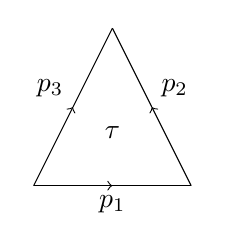
\begin{tikzpicture}
        \draw[->] (-1,0) -- (0, 0) node[below]{$p_1$};
        \draw (0, 0) -- (1, 0);
        \draw[->] (1,0) -- (0.5, 1) node[above right]{$p_2$};
        \draw (0.5, 1) -- (0, 2);
        \draw[->] (-1,0) -- (-0.5, 1) node[above left]{$p_3$};
        \draw (-0.5, 1) -- (0, 2);
        \draw (0, 0.67) node{$\tau$};
    \end{tikzpicture}
\end{figure}

We can continue in this manner with higher-dimensional simplices. Surprise surprise, they form a chain complex: indeed, in the above case
\begin{cd*}
    \R^{\+ T} \arrow[r, "\del"] & \R^{\+ P} \arrow[r, "\del"] & \R^{\+ X}
\end{cd*}
we can see that $\del^2(\tau) = 0$ for all $\tau$, because $p_1 + p_2 - p_3$ is a loop (so its start point minus its end point is zero). We can show something analogous when we consider boundary maps between free modules generated by paths from higher-dimensional simplices as well.

We can thus compute homology as usual:
\begin{align*}
    H_n\of{X; \R} := \quotient{\pker{\del}}{\pim{\del}}
\end{align*}
(and similarly for $H_n\of{X; R}$ where $R$ is any commutative ring).

\subsection{A Formal Definition (of Singular Homology)}

We begin by defining the $n$-simplex.

\begin{boxdefinition}[$n$-Simplex]
    For all $n \in \N$, define the \textbf{$n$-simplex} to be the following subset of $\R^n$:
    \begin{align*}
        \Delta^n := \setst{x \in \R^{n}}{\sum_{i=1}^{n} x_i = 1 \text{ and } \forall i, \ x_i \geq 0}
    \end{align*}
\end{boxdefinition}

Simplices are well-understood, particularly in low dimensions:
\begin{enumerate}
    \item The $0$-simplex is a point.
    \item The $1$-simplex is a line.
    \item The $2$-simplex is a triangle.
    \item The $3$-simplex is a tetrahedron.
\end{enumerate}

\begin{boxdefinition}[Singular $n$-Simplex]
    Let $X$ be a topological space. A continuous map $\sigma : \Delta^n \to X$ is called a \textbf{singular $n$-simplex}.
\end{boxdefinition}

For the remainder of this subsection, let $G$ denote an additively expressed abelian group. Unless otherwise specified, $G$ will denote the integers.

\begin{boxdefinition}[Group of $n$-Chains]
    For all $n \in \N$, define the \textbf{group of $n$-chains $C_n\of{X; G}$} to be the group whose elements are formal finite linear combinations $\sum_{i=1}^{k} \lambda_i \sigma_i$ of singular $n$-simplices $\sigma_i : \Delta^n \to X$ with coefficients $\lambda_i \in G$.
\end{boxdefinition}

Before proceeding any further, we introduce some notation.

\begin{boxnotation}
    We denote by $\brac{v_0, \ldots, \widehat{v_i}, \ldots, v_n}$ the tuple $\brac{v_0, \ldots, v_{i-1}, v_{i+1}, \ldots, v_n}$.
\end{boxnotation}

Now, we define the boundary map.

\begin{boxdefinition}[Boundary Map]
    We let $\partial_n:C_n(X;G)\rightarrow C_{n-1}(X;G)$ denote the ($n^{th}$) \textbf{boundary map}, where $\partial_n$ is defined on a basis of $C_n(X;G)$ by $$\partial_n(\sigma):=\sum_{i=0}^n (-1)^i\sigma\restriction_{[v_0, \ldots, \widehat{v_i}, \ldots, v_n]}$$ where $[v_0, \ldots, v_n]$ is set of vertices of $\triangle^n$ (i.e. standard basis of $\R^n$).
\end{boxdefinition}

The kernel of the boundary map consists of all cycles and the image consists of all boundaries.

\begin{boxlemma}
    $\del_n \circ \del_{n + 1} = 0$.
\end{boxlemma}
\begin{proof}
    Fix $\sigma \in C_n\of{X; G}$. We have
    \begin{align*}
        \del_n\of{\del_{n+1}(\sigma)}
        &= \del_n\of{\sum_{i=0}^{n+1} \parenth{-1}^{i} \cdot \sigma\vert_{\brac{v_0, \ldots, \widehat{v_i}, \ldots, v_{n+1}}}} \\
        &= \sum_{i=0}^{n+1} \sum_{j < i} \parenth{-1}^i \parenth{-1}^j \cdot \sigma\vert_{\brac{v_0, \ldots, \widehat{v_j}, \ldots, \widehat{v_i}, \ldots, v_{n+1}}}
        +
        \sum_{i=0}^{n+1} \sum_{j > i} \parenth{-1}^i \parenth{-1}^{j-1} \cdot \sigma\vert_{\brac{v_0, \ldots, \widehat{v_i}, \ldots, \widehat{v_j}, \ldots, v_{n+1}}} \\
        &= \sum_{i=0}^{n+1} \sum_{j < i} \parenth{-1}^i \parenth{-1}^j \cdot \sigma\vert_{\brac{v_0, \ldots, \widehat{v_j}, \ldots, \widehat{v_i}, \ldots, v_{n+1}}}
        +
        \sum_{j=0}^{n+1} \sum_{i > j} \parenth{-1}^{j} \parenth{-1}^{i-1} \cdot \sigma\vert_{\brac{v_0, \ldots, \widehat{v_j}, \ldots, \widehat{v_i}, \ldots, v_{n+1}}} \\
        &= 0
    \end{align*}
    Thus, $\del_n \circ \del_{n+1} = 0$.
\end{proof}

Thus, $\pim{\del_n} \ssq \pim{\del_{n+1}}$, and the following is a chain complex in the category of abelian groups:
\begin{cd}
    \cdots \arrow[r]
    & C_{n+1}\of{X; G} \arrow[r, "\del_{n+1}"]
    & C_n\of{X; G} \arrow[r, "\del_n"]
    & C_{n-1}\of{X; G} \arrow[r, "\del_{n-1}"]
    & \cdots
    \label{Ch2:CD:Chain_Complex_Cycles}
\end{cd}

\begin{boxdefinition}[Cycles]
    We define a \textbf{cycle} in $C_n\of{X; G}$ to be an element of $\pker{\del_n}$. We denote $Z_n\of{X; G} := \pker{\del_n}$.
\end{boxdefinition}

\begin{boxdefinition}[Boundary Elements]
    We define a \textbf{boundary element} of $C_{n-1}\of{X; G}$ to be an element of $\pim{\del_n}$. We denote $B_n\of{X; G} := \pim{\del_n}$.
\end{boxdefinition}

We are now finally ready to define the $n$th homology group of topological space.

\begin{boxdefinition}[$n$th Homology Group]
    We define the \textbf{$n$th homology group of $X$ with respect to $G$} to be the quotient group
    \begin{align*}
        H_n\of{X; G} := \quotient{\pker{\del_n}}{\pim{\del_{n+1}}} = \quotient{Z_n\of{X;G}}{B_{n+1}\of{X;G}}
    \end{align*}
\end{boxdefinition}

% Note that we can analogously define \textbf{simplicial homology}, where we divide a space into simplices and 

We can also define
\begin{itemize}
    \item \textbf{simplicial homology}, where we divide a space into simplices and proceed geometrically. This coincides with singular homology.
    \item \textbf{reduced homology}, which is exactly the same as singular homology except at index $0$, where we define the boundary map to go from $C_0\of{X; G}$ to $G$ in a way that sends every $\sigma$ to $1$.
\end{itemize}

As we would expect, homology is functorial. As a first step, we show that continuous maps induce morphisms of chain complexes on the chains of cycles. Then, as we know and love, we apply the fact that chain complex morphisms induce homology morphisms.

Moreover, as we would expect, under this correspondence, a homotopy equivalence of topological spaces maps to a homotopy equivalence of chain complexes, which results in an isomorphism on homology.

Finally (as is obvious from functoriality), if we have a homeomorphism, then we get a chain complex isomorphism, and subsequently an isomorphism of homology groups.
\section{Complex Structures}

Let $X$ be a topological space.

\begin{boxdefinition}[$\Delta$-complex]
    A $\Delta$-complex structure on $X$ is a set of singular $n$-simplices $\delta_{\alpha} : '\Delta^n \to X$ for varying $n = n(\alpha)$ such that
    \begin{enumerate}
        \item every $x \in X$ is the image of at least one $\delta_{\alpha}$, $\sigma_{\alpha} \vert_{\interior{\Delta^n}}$ is injective
        \item $\sigma_{\alpha}\vert_{\brac{v_0, \ldots, \widehat{v_i}, \ldots, v_n}}$ is $\sigma_{\beta} : \Delta^{k-1} \to X$ in the order-preserving identification of vertices
        \item $U \ssq X$ is open iff $\sigma_{\alpha}\inv\of{U}$ is open for all $\alpha$.
    \end{enumerate}
\end{boxdefinition}

This is the ``minimal definition'' for making the definition of homology work.

Our objective will be to show that homotopies of spaces induce homotopies of chain complexes.

\subsection{Prisms}

\begin{boxdefinition}[$n$-Prism]
    For all $n \in \N$, define the $n$-prism to be $\Delta^n \times I \ssq \R^n$.
\end{boxdefinition}

This is not a simplex, so we need to triangulate: we can view the $n$-prism as a(n uncountable) union of $(n-1)$-simplices. Denote the bottom $n$-simplex of an $n$-prism by $v_0, \ldots, v_n$ and the top $n$-simplex by $w_0, \ldots, w_n$.

\begin{boxdefinition}[Prism Operator]
    Define $P : C_n(X) \to C_{n+1}(X)$ by
    \begin{align*}
        P(\sigma) = \sum_{i} (-1)^{i} F \circ (\sigma \times \id) \vert_{\brac{v_0, \ldots, v_i, w_i, \ldots, w_n}}
    \end{align*}
\end{boxdefinition}

\begin{boxproposition}
    Given $f, g : X \to Y$, if
    \begin{align*}
        \del \circ P = g_{\#} - f_{\#} - P \circ \del
    \end{align*}
    then the maps induced by $f$ and $g$ on homology
    \begin{align*}
        f_*, g_* : H_*(X) \to H_*(Y)
    \end{align*}
    are equal.
\end{boxproposition}

\begin{boxdefinition}[Chain Homotopy]
    A sequence of maps $P_n : C_n(X) \to C_{n+1}(X)$ is called a \textbf{chain homotopy} if
    \begin{align*}
        \del \circ P + P \circ \del = g_{\#} - f_{\#}
    \end{align*}
\end{boxdefinition}

We keep in mind the following commutative diagram:
\begin{cd*}
    \cdots &[2em] {C_{n+1}(X)} &[4em] {C_n(X)} &[4em] {C_{n-1}(X)} &[2em] \cdots \\[4em]
	\cdots &[2em] {C_{n+1}(X)} &[4em] {C_n(Y)} &[4em] {C_{n-1}(X)} &[2em] \cdots
	\arrow["\partial", from=1-1, to=1-2]
	\arrow["\partial", from=1-2, to=1-3]
	\arrow["{f_{\#}}"', shift right, from=1-2, to=2-2]
	\arrow["{g_{\#}}", shift left, from=1-2, to=2-2]
	\arrow["\partial", from=1-3, to=1-4]
	\arrow["P"{description}, from=1-3, to=2-2]
	\arrow["{f_{\#}}"', shift right, from=1-3, to=2-3]
	\arrow["{g_{\#}}", shift left, from=1-3, to=2-3]
	\arrow["\partial", from=1-4, to=1-5]
	\arrow["P"{description}, from=1-4, to=2-3]
	\arrow["{g_{\#}}", shift left, from=1-4, to=2-4]
	\arrow["{f_{\#}}"', shift right, from=1-4, to=2-4]
	\arrow["\partial"', from=2-1, to=2-2]
	\arrow["\partial"', from=2-2, to=2-3]
	\arrow["\partial"', from=2-3, to=2-4]
	\arrow["\partial"', from=2-4, to=2-5]
\end{cd*}

\subsection{Exact Sequences}

Let $A \ssq X$. By $C_n(A)$, we denote the group $C_n(A; \Z)$ - the free abelian group generated by continuous functions from $\Delta^n$ to $A$.

It is, of course, a subgroup of $C_n(X)$, and since everything is abelian, all subgroups are normal, so we can construct a chain complex of quotients
\begin{align*}
    C_n\of{X, A} := \quotient{C_n(X)}{C_n(A)}
\end{align*}
\begin{boxtheorem}[Zigzag Theorem/Long Exact Sequence of Homology]\label{SP:Thm:LES_Homology}
    A short exact sequence $0\rightarrow A_{*}\rightarrow B_{*}\rightarrow C_{*} \to 0$ of chain complexes induces a long exact sequence of homology groups.
    % \begin{cd*}
    %     \cdots 
    %     \arrow[r] 
    %     & H_n(A) 
    %     \arrow[r] 
    %     & H_n(B) 
    %     \arrow[r] 
    %     & H_n(C) 
    %     \arrow[dll, 
    %          decorate,
    %          decoration={snake, amplitude=1.2pt, segment length=6pt},
    %          "\delta_n"'] \\
    %     H_{n-1}(A) 
    %     \arrow[r] 
    %     & H_{n-1}(B) 
    %     \arrow[r] 
    %     & H_{n-1}(C) 
    %     \arrow[dll, 
    %          decorate,
    %          decoration={snake, amplitude=1.2pt, segment length=6pt},
    %          "\delta_{n-1}"'] \\
    %     H_{n-2}(A) 
    %     \arrow[r] 
    %     & H_{n-2}(B) 
    %     \arrow[r] 
    %     & H_{n-2}(C) 
    %     \arrow[r] 
    %     & \cdots
    % \end{cd*}
\end{boxtheorem}
\begin{proof}
    See \cite[Week 6, Lemma 1.6]{ICLAlg4} for a proof that uses the Snake Lemma or \cite[Proposition 5.5.1]{EPFLRingsAndModules} for a more fleshed out version.
\end{proof}

Recall the following definition.

\begin{boxdefinition}
    For $A \ssq X$, we denote by $C_{\bullet}(X, A)$ the chain complex given by
    \begin{align*}
        C_n(X, A) = \quotient{C_n(X)}{C_n(A)}
    \end{align*}
    for all $n \in \N$.
\end{boxdefinition}

\begin{boxtheorem}[Long Exact Sequence of a Pair]
    For all $A \ssq X$, there is a LES
    \begin{cd*}
        \cdots \arrow[r] & H_n(A) \arrow[r] & H_n(X) \arrow[r] & H_n(X, A) \arrow[r] & H_{n-1}(A) \arrow[r] & \cdots
    \end{cd*}
\end{boxtheorem}
\begin{proof}
    Exactly \Cref{SP:Thm:LES_Homology} applied to the SES
    \begin{cd*}
        0 \arrow[r] & C_{\bullet}\of{A} \arrow[r] & C_{\bullet}\of{X} \arrow[r] & C_{\bullet}\of{X, A} \arrow[r] & 0
    \end{cd*}
\end{proof}
Say now that we have a space $X=A\cup B$ for some open $A,B$. We would like to say that $0\rightarrow C_n(A\cap B)\rightarrow C_n(A)\oplus C_n(B)\rightarrow C_n(X)\rightarrow 0$ is short exact, but this is not quite true - we can imagine a simplex $S$ which is only partially contained in each of $A,B$. However there is an easy fix for this (and it is what you would expect).

\begin{boxnotation}
    Let $X$ be a space that is covered by open sets $A$ and $B$. Define
    \begin{align*}
        C^{\set{A, B}}_n(X)
    \end{align*}
    to be the subgroup of $C_n(X)$ generated by those $\sigma : \Delta^n \to X$ such that $\pim{\sigma} \ssq A$ or $\pim{\sigma} \ssq B$.
\end{boxnotation}

The idea of the above is that we are somehow ``splitting simplices into two parts''---the part contained in $A$ and the part conained in $B$.

\begin{boxtheorem}
    Given a space $X$ and open sets $A, B \ssq X$ such that $X = A \cup B$, the following is a short exact sequence of chain complexes:
    \begin{cd*}
        0 \arrow[r] & C_{*}\of{A \cap B} \arrow[r] & C_{*}(A) \+ C_{*}(B) \arrow[r] & C^{\set{A, B}}_{*}(X) \arrow[r] & 0
    \end{cd*}
\end{boxtheorem}

Note that in the above SES, if we were to replace $C_{*}^{\set{A, B}}(X)$ by $C_{*}(X)$, the sequence would cease to be exact.

\begin{boxlemma}
    For all $n \in \N$, the $n$th homology group of $C_{*}(X)$ is the same as the $n$th homology group of $C_{*}^{\set{A, B}}(X)$.
\end{boxlemma}

More generally, we show the following.

\begin{boxlemma}
    Let $\U = \setst{U_j \ssq X}{j < J}$ be subsets of $X$ whose interiors cover $X$. Define
    \begin{align*}
        C_n^{\U}(X) := \setst{\sum_i \lambda_i \sigma_i \in C_n(X)}{\forall i,\ \exists j \st \pim{\sigma_i} \ssq U_j}
    \end{align*}
    The inclusions $i_{*} : C_{*}^{\U}(X) \inj C_{*}(X)$ form a homotopy equivalence of chain complexes.
\end{boxlemma}

By the Zigzag theorem, this gives an LES in homology:
\begin{boxdefinition}[Mayer-Vietoris Sequence]
    Given $X$ covered by the interiors of two sets $A,B$ we call the LES
    \begin{cd*}
        \cdots \arrow[r]
        &[0.1em] H_n\of{A \cap B} \arrow[r]
        & H_n(A) \+ H_n(B) \arrow[r]
        & H_n(X) \arrow[r]
        & H_{n-1}\of{A \cap B} \arrow[r]
        % & H_{n-1}(A) \+ H_{n-1}(B) \arrow[r]
        &[0.1em] \cdots
    \end{cd*}
    the \textbf{Mayer-Vietoris Sequence for $X$}.
\end{boxdefinition}

Say we have a space $X$ and $\mathcal{U}=\{U_j:j\in J\}$ is a cover of $X$ and the interiors of the $U_j$ also cover $X$. We let $C_n^{\mathcal{U}}\ssq C_n(X)$ consist of all chains $\sum_{i\in I} \lambda_i \sigma_i$ where for all $i\in I$ we have $\text{im}(\sigma_i)\ssq U_j$ for some $j$. Note that the boundary maps $\partial$ restrict to boundary maps $\partial: C_n{\mathcal{U}}\rightarrow C_{n-1}^{\mathcal{U}}(X)$. 

We now temporarily call the corresponding homology groups $H_n^{\mathcal{U}}(X)$ (``temporarily'' because we will hopefully soon show that $H_n^{\mathcal{U}}(X)$ is just $H_n(X)$ for every $\mathcal{U}$):
\begin{boxlemma}
    The inclusion map $i:C_n^{\mathcal{U}}(X)\rightarrow C_n(X)$ is a chain homotopy equivalence (i.e. the projection $p:C_n(X)\rightarrow C_n^{\mathcal{U}}(X)$ is such that $p\circ i$ and $i\circ p$ are chain homotopic to the identity), and in particular we have $H_n^{\mathcal{U}}(X)\cong H_n(X)$.
\end{boxlemma}
\begin{proof}
    We just split $\Delta^n$ into many smaller simplices, for example by repeated barycentric subdivisions... we then find a homotopy of chain complexes between $C_{*}(X)$ and $C_{*}^{\set{A, B}}(X)$.

    Let $Y \ssq \R^d$ be a convex set, and let $LC_n(Y) \ssq C_n(Y)$ denote the subgroup of affine maps $\sigma : \Delta^n \to Y$. The boundary map $\partial$ restricts to a map $\partial : LC_n(Y) \to LC_{n-1}(Y)$. For every $b \in Y$, define
    \begin{align*}
        b : LC_n(Y) \to LC_{n+1}(Y) : \brac{w_0, \dots, w_n} \mapsto \brac{b, w_0, \ldots, w_n}
    \end{align*}
    It is not difficult to show that
    \begin{align*}
        \partial \circ b = \id - b \circ \partial \iff \partial \circ b + b \circ \partial = \id
    \end{align*}

    We now let $S:LC_n(Y)\rightarrow LC_n(Y)$ be defined inductively by $S:LC_0(Y)\rightarrow LC_0(Y)$ is the identity, and $S_{\sigma}=b_{\sigma}(S\partial \sigma)$, where $B_{\sigma}$ is the barycenter of $S\partial \sigma$. Then $\partial S_{\sigma}=\partial b_{\sigma}(S\partial \sigma)=S\partial \sigma -b_{\sigma}\partial $\sorry
\end{proof}

\subsection{Application: Homology Groups of Spheres}

Let $B_n$ denote the closed unit ball in $\R^n$ centred at the origin, so that $S^{n-1} = \partial B_n \subseteq B_n$. Then, the following is a long exact sequence:
\begin{cd*}
    \cdots \arrow[r] & H_k\of{S^{n-1}} \arrow[r] & H_k\of{B_n} \arrow[r] & H_k\of{B_n, S^{n-1}} \arrow[r] & H_{k-1}\of{S^{n-1}} \arrow[r] & \cdots
\end{cd*}

We can show the following fact.

\begin{boxtheorem}
    $H_n\of{S^n; \Z} \cong \Z$ for all $n \geq 1$.
\end{boxtheorem}
\begin{proof}
    
\end{proof}

% Next up: Mayer-Vietoris

\subsection{Excision}

(Recall that relative homology is obtained by quotienting out chain complexes in $X$ by chain complexes in $A$ and then computing homology.)

\begin{boxtheorem}[Excision]
    Let $A, B \ssq X$, with the interiors covering $X$. The inclusion of $(B, A \cap B)$ into $(X, A)$ induces isomorphisms
    \begin{align*}
        H_ n\of{B, A \cap B} \xrightarrow{\sim} H_n\of{X, A}
    \end{align*}
    for all $n \in \N$. Equivalently, suppose we have a chain of inclusions $Z \ssq A \ssq X$, with $\cl{Z} \ssq \interior{A}$. Then,
    \begin{align*}
        H_n(X, A) \cong H_n\of{X \setminus Z, A \setminus Z}
    \end{align*}
    These equivalent phenomena are called \textbf{excision}.
\end{boxtheorem}
\begin{proof}
    We have a diagram
    \begin{cd*}
        \quotient{C_n(B)}{C_n(A \cap B)} \arrow[r] &
        \quotient{C_n^{\set{A, B}}(X)}{C_n(A)} \arrow[r, "\text{induces isomorphism on $H_*$}"] &[8em]
        \quotient{C_n(X)}{C_n(A)}
    \end{cd*}
\end{proof}